\documentclass[1p]{elsarticle_modified}
%\bibliographystyle{elsarticle-num}

%\usepackage[colorlinks]{hyperref}
%\usepackage{abbrmath_seonhwa} %\Abb, \Ascr, \Acal ,\Abf, \Afrak
\usepackage{amsfonts}
\usepackage{amssymb}
\usepackage{amsmath}
\usepackage{amsthm}
\usepackage{scalefnt}
\usepackage{amsbsy}
\usepackage{kotex}
\usepackage{caption}
\usepackage{subfig}
\usepackage{color}
\usepackage{graphicx}
\usepackage{xcolor} %% white, black, red, green, blue, cyan, magenta, yellow
\usepackage{float}
\usepackage{setspace}
\usepackage{hyperref}

\usepackage{tikz}
\usetikzlibrary{arrows}

\usepackage{multirow}
\usepackage{array} % fixed length table
\usepackage{hhline}

%%%%%%%%%%%%%%%%%%%%%
\makeatletter
\renewcommand*\env@matrix[1][\arraystretch]{%
	\edef\arraystretch{#1}%
	\hskip -\arraycolsep
	\let\@ifnextchar\new@ifnextchar
	\array{*\c@MaxMatrixCols c}}
\makeatother %https://tex.stackexchange.com/questions/14071/how-can-i-increase-the-line-spacing-in-a-matrix
%%%%%%%%%%%%%%%

\usepackage[normalem]{ulem}

\newcommand{\msout}[1]{\ifmmode\text{\sout{\ensuremath{#1}}}\else\sout{#1}\fi}
%SOURCE: \msout is \stkout macro in https://tex.stackexchange.com/questions/20609/strikeout-in-math-mode

\newcommand{\cancel}[1]{
	\ifmmode
	{\color{red}\msout{#1}}
	\else
	{\color{red}\sout{#1}}
	\fi
}

\newcommand{\add}[1]{
	{\color{blue}\uwave{#1}}
}

\newcommand{\replace}[2]{
	\ifmmode
	{\color{red}\msout{#1}}{\color{blue}\uwave{#2}}
	\else
	{\color{red}\sout{#1}}{\color{blue}\uwave{#2}}
	\fi
}

\newcommand{\Sol}{\mathcal{S}} %segment
\newcommand{\D}{D} %diagram
\newcommand{\A}{\mathcal{A}} %arc


%%%%%%%%%%%%%%%%%%%%%%%%%%%%%5 test

\def\sl{\operatorname{\textup{SL}}(2,\Cbb)}
\def\psl{\operatorname{\textup{PSL}}(2,\Cbb)}
\def\quan{\mkern 1mu \triangleright \mkern 1mu}

\theoremstyle{definition}
\newtheorem{thm}{Theorem}[section]
\newtheorem{prop}[thm]{Proposition}
\newtheorem{lem}[thm]{Lemma}
\newtheorem{ques}[thm]{Question}
\newtheorem{cor}[thm]{Corollary}
\newtheorem{defn}[thm]{Definition}
\newtheorem{exam}[thm]{Example}
\newtheorem{rmk}[thm]{Remark}
\newtheorem{alg}[thm]{Algorithm}

\newcommand{\I}{\sqrt{-1}}
\begin{document}

%\begin{frontmatter}
%
%\title{Boundary parabolic representations of knots up to 8 crossings}
%
%%% Group authors per affiliation:
%\author{Yunhi Cho} 
%\address{Department of Mathematics, University of Seoul, Seoul, Korea}
%\ead{yhcho@uos.ac.kr}
%
%
%\author{Seonhwa Kim} %\fnref{s_kim}}
%\address{Center for Geometry and Physics, Institute for Basic Science, Pohang, 37673, Korea}
%\ead{ryeona17@ibs.re.kr}
%
%\author{Hyuk Kim}
%\address{Department of Mathematical Sciences, Seoul National University, Seoul 08826, Korea}
%\ead{hyukkim@snu.ac.kr}
%
%\author{Seokbeom Yoon}
%\address{Department of Mathematical Sciences, Seoul National University, Seoul, 08826,  Korea}
%\ead{sbyoon15@snu.ac.kr}
%
%\begin{abstract}
%We find all boundary parabolic representation of knots up to 8 crossings.
%
%\end{abstract}
%\begin{keyword}
%    \MSC[2010] 57M25 
%\end{keyword}
%
%\end{frontmatter}

%\linenumbers
%\tableofcontents
%
\newcommand\colored[1]{\textcolor{white}{\rule[-0.35ex]{0.8em}{1.4ex}}\kern-0.8em\color{red} #1}%
%\newcommand\colored[1]{\textcolor{white}{ #1}\kern-2.17ex	\textcolor{white}{ #1}\kern-1.81ex	\textcolor{white}{ #1}\kern-2.15ex\color{red}#1	}

{\Large $\underline{12n_{0393}~(K12n_{0393})}$}

\setlength{\tabcolsep}{10pt}
\renewcommand{\arraystretch}{1.6}
\vspace{1cm}\begin{tabular}{m{100pt}>{\centering\arraybackslash}m{274pt}}
\multirow{5}{120pt}{
	\centering
	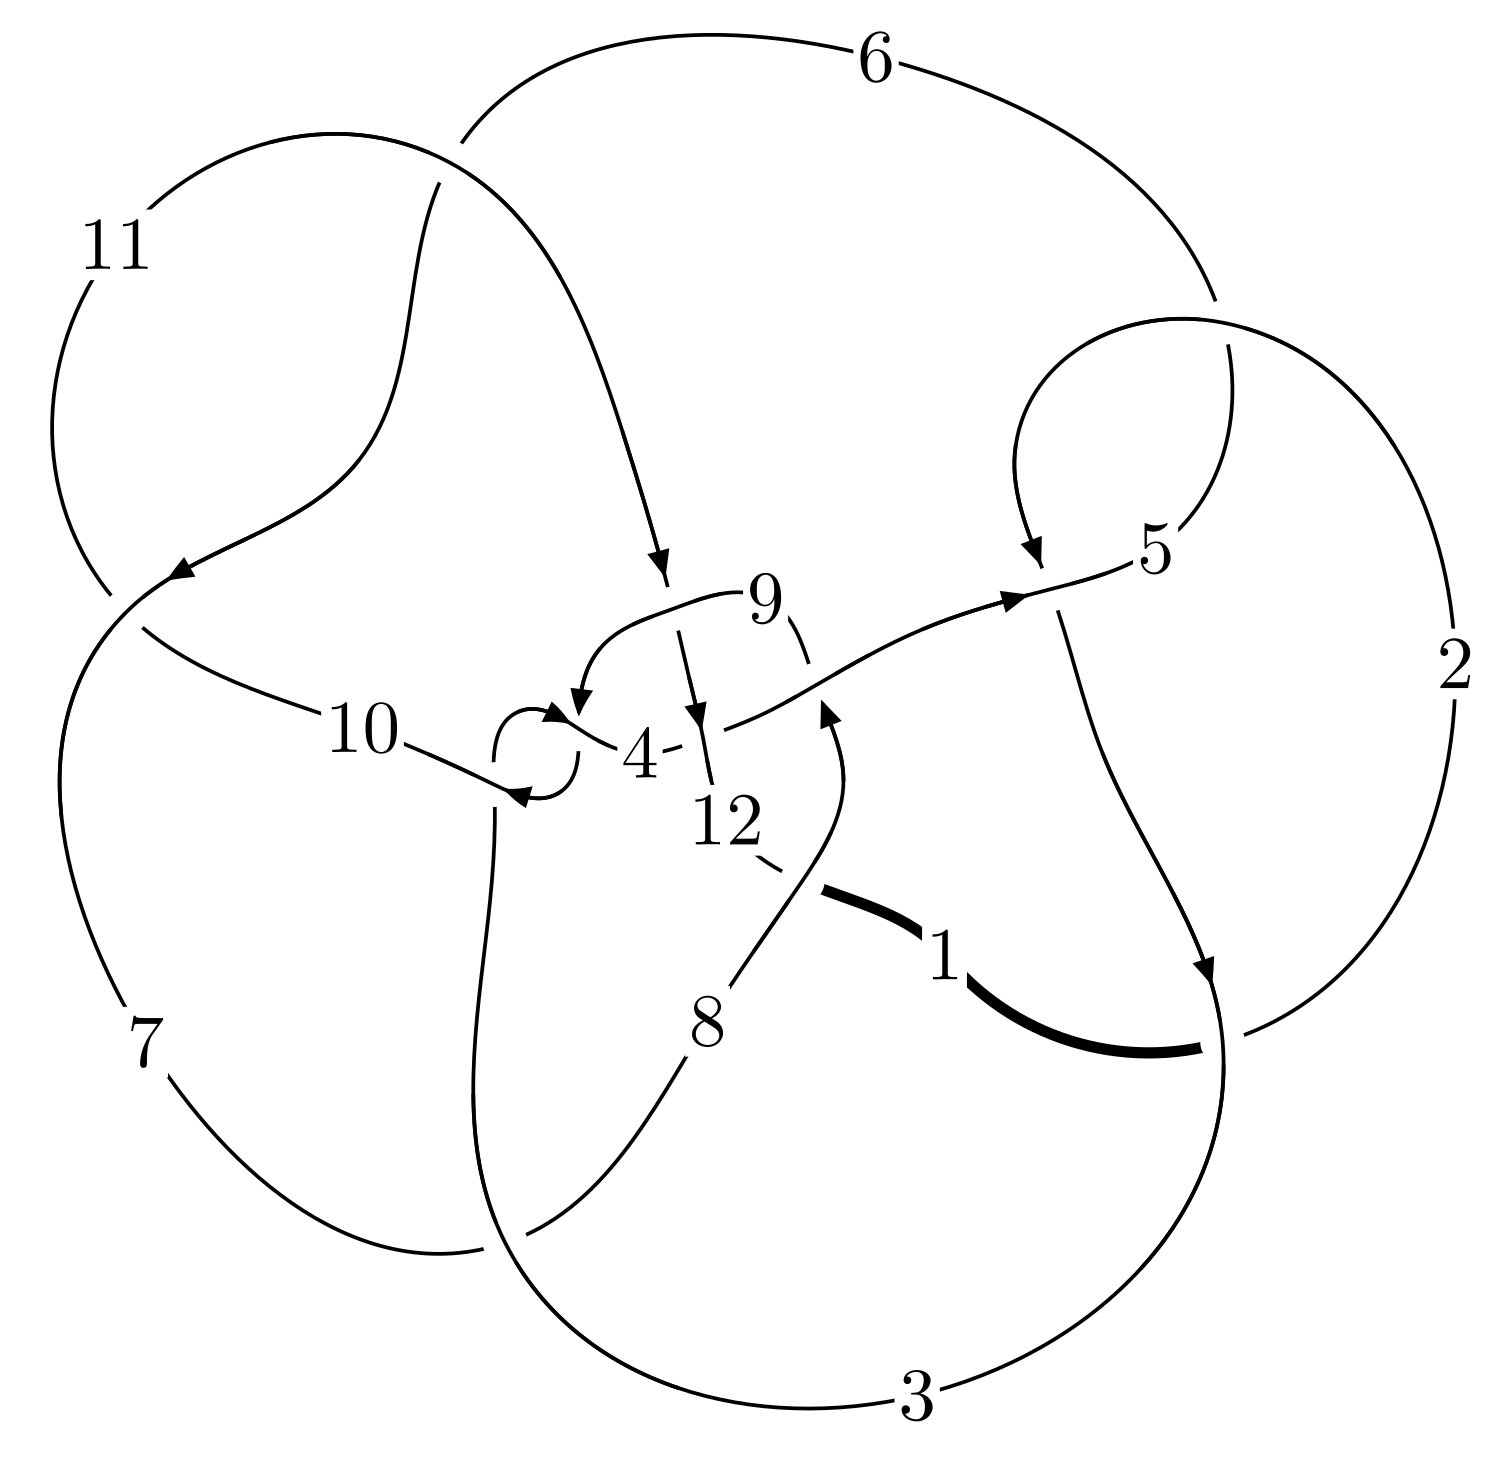
\includegraphics[width=112pt]{../../../GIT/diagram.site/Diagrams/png/2482_12n_0393.png}\\
\ \ \ A knot diagram\footnotemark}&
\allowdisplaybreaks
\textbf{Linearized knot diagam} \\
\cline{2-2}
 &
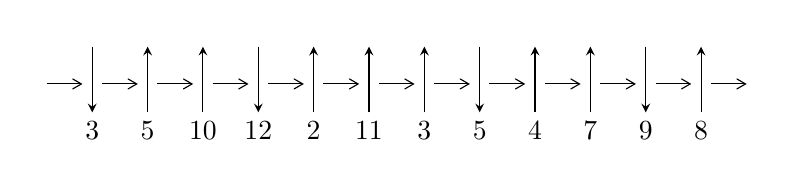
\begin{tikzpicture}[x=20pt, y=17pt]
	% nodes
	\node (C0) at (0, 0) {};
	\node (C1) at (1, 0) {};
	\node (C1U) at (1, +1) {};
	\node (C1D) at (1, -1) {3};

	\node (C2) at (2, 0) {};
	\node (C2U) at (2, +1) {};
	\node (C2D) at (2, -1) {5};

	\node (C3) at (3, 0) {};
	\node (C3U) at (3, +1) {};
	\node (C3D) at (3, -1) {10};

	\node (C4) at (4, 0) {};
	\node (C4U) at (4, +1) {};
	\node (C4D) at (4, -1) {12};

	\node (C5) at (5, 0) {};
	\node (C5U) at (5, +1) {};
	\node (C5D) at (5, -1) {2};

	\node (C6) at (6, 0) {};
	\node (C6U) at (6, +1) {};
	\node (C6D) at (6, -1) {11};

	\node (C7) at (7, 0) {};
	\node (C7U) at (7, +1) {};
	\node (C7D) at (7, -1) {3};

	\node (C8) at (8, 0) {};
	\node (C8U) at (8, +1) {};
	\node (C8D) at (8, -1) {5};

	\node (C9) at (9, 0) {};
	\node (C9U) at (9, +1) {};
	\node (C9D) at (9, -1) {4};

	\node (C10) at (10, 0) {};
	\node (C10U) at (10, +1) {};
	\node (C10D) at (10, -1) {7};

	\node (C11) at (11, 0) {};
	\node (C11U) at (11, +1) {};
	\node (C11D) at (11, -1) {9};

	\node (C12) at (12, 0) {};
	\node (C12U) at (12, +1) {};
	\node (C12D) at (12, -1) {8};
	\node (C13) at (13, 0) {};

	% arrows
	\draw[->,>={angle 60}]
	(C0) edge (C1) (C1) edge (C2) (C2) edge (C3) (C3) edge (C4) (C4) edge (C5) (C5) edge (C6) (C6) edge (C7) (C7) edge (C8) (C8) edge (C9) (C9) edge (C10) (C10) edge (C11) (C11) edge (C12) (C12) edge (C13) ;	\draw[->,>=stealth]
	(C1U) edge (C1D) (C2D) edge (C2U) (C3D) edge (C3U) (C4U) edge (C4D) (C5D) edge (C5U) (C6D) edge (C6U) (C7D) edge (C7U) (C8U) edge (C8D) (C9D) edge (C9U) (C10D) edge (C10U) (C11U) edge (C11D) (C12D) edge (C12U) ;
	\end{tikzpicture} \\
\hhline{~~} \\& 
\textbf{Solving Sequence} \\ \cline{2-2} 
 &
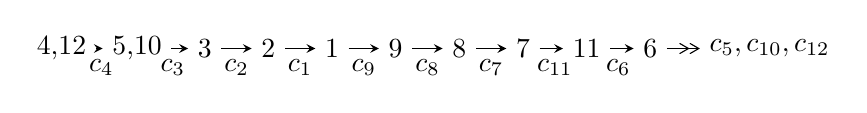
\begin{tikzpicture}[x=23pt, y=7pt]
	% node
	\node (A0) at (-1/8, 0) {4,12};
	\node (A1) at (17/16, 0) {5,10};
	\node (A2) at (17/8, 0) {3};
	\node (A3) at (25/8, 0) {2};
	\node (A4) at (33/8, 0) {1};
	\node (A5) at (41/8, 0) {9};
	\node (A6) at (49/8, 0) {8};
	\node (A7) at (57/8, 0) {7};
	\node (A8) at (65/8, 0) {11};
	\node (A9) at (73/8, 0) {6};
	\node (C1) at (1/2, -1) {$c_{4}$};
	\node (C2) at (13/8, -1) {$c_{3}$};
	\node (C3) at (21/8, -1) {$c_{2}$};
	\node (C4) at (29/8, -1) {$c_{1}$};
	\node (C5) at (37/8, -1) {$c_{9}$};
	\node (C6) at (45/8, -1) {$c_{8}$};
	\node (C7) at (53/8, -1) {$c_{7}$};
	\node (C8) at (61/8, -1) {$c_{11}$};
	\node (C9) at (69/8, -1) {$c_{6}$};
	\node (A10) at (11, 0) {$c_{5},c_{10},c_{12}$};

	% edge
	\draw[->,>=stealth]	
	(A0) edge (A1) (A1) edge (A2) (A2) edge (A3) (A3) edge (A4) (A4) edge (A5) (A5) edge (A6) (A6) edge (A7) (A7) edge (A8) (A8) edge (A9) ;
	\draw[->>,>={angle 60}]	
	(A9) edge (A10);
\end{tikzpicture} \\ 

\end{tabular} \\

\footnotetext{
The image of knot diagram is generated by the software ``\textbf{Draw programme}" developed by Andrew Bartholomew(\url{http://www.layer8.co.uk/maths/draw/index.htm\#Running-draw}), where we modified some parts for our purpose(\url{https://github.com/CATsTAILs/LinksPainter}).
}\phantom \\ \newline 
\centering \textbf{Ideals for irreducible components\footnotemark of $X_{\text{par}}$} 
 
\begin{align*}
I^u_{1}&=\langle 
1.15453\times10^{112} u^{51}+5.72428\times10^{112} u^{50}+\cdots+1.21115\times10^{113} b-3.01826\times10^{112},\\
\phantom{I^u_{1}}&\phantom{= \langle  }-2.72037\times10^{112} u^{51}+1.17488\times10^{112} u^{50}+\cdots+3.63345\times10^{113} a+5.57200\times10^{113},\\
\phantom{I^u_{1}}&\phantom{= \langle  }u^{52}+3 u^{51}+\cdots-24 u+3\rangle \\
I^u_{2}&=\langle 
2.01791\times10^{18} u^{27}-2.77559\times10^{18} u^{26}+\cdots+3.98012\times10^{18} b-1.63190\times10^{18},\\
\phantom{I^u_{2}}&\phantom{= \langle  }2.25156\times10^{18} u^{27}-4.18384\times10^{18} u^{26}+\cdots+3.98012\times10^{18} a-1.75552\times10^{19},\;u^{28}-2 u^{27}+\cdots-2 u+1\rangle \\
\\
\end{align*}
\raggedright * 2 irreducible components of $\dim_{\mathbb{C}}=0$, with total 80 representations.\\
\footnotetext{All coefficients of polynomials are rational numbers. But the coefficients are sometimes approximated in decimal forms when there is not enough margin.}
\newpage
\renewcommand{\arraystretch}{1}
\centering \section*{I. $I^u_{1}= \langle 1.15\times10^{112} u^{51}+5.72\times10^{112} u^{50}+\cdots+1.21\times10^{113} b-3.02\times10^{112},\;-2.72\times10^{112} u^{51}+1.17\times10^{112} u^{50}+\cdots+3.63\times10^{113} a+5.57\times10^{113},\;u^{52}+3 u^{51}+\cdots-24 u+3 \rangle$}
\flushleft \textbf{(i) Arc colorings}\\
\begin{tabular}{m{7pt} m{180pt} m{7pt} m{180pt} }
\flushright $a_{4}=$&$\begin{pmatrix}1\\0\end{pmatrix}$ \\
\flushright $a_{12}=$&$\begin{pmatrix}0\\u\end{pmatrix}$ \\
\flushright $a_{5}=$&$\begin{pmatrix}1\\u^2\end{pmatrix}$ \\
\flushright $a_{10}=$&$\begin{pmatrix}0.0748701 u^{51}-0.0323350 u^{50}+\cdots-79.8705 u-1.53353\\-0.0953248 u^{51}-0.472631 u^{50}+\cdots-14.8071 u+0.249205\end{pmatrix}$ \\
\flushright $a_{3}=$&$\begin{pmatrix}0.434214 u^{51}+1.30766 u^{50}+\cdots+80.9069 u-0.00257423\\0.125422 u^{51}+0.440759 u^{50}+\cdots+12.0661 u-0.102321\end{pmatrix}$ \\
\flushright $a_{2}=$&$\begin{pmatrix}0.449835 u^{51}+1.36244 u^{50}+\cdots+67.6586 u+0.0846844\\0.136943 u^{51}+0.472556 u^{50}+\cdots+12.2091 u-0.126050\end{pmatrix}$ \\
\flushright $a_{1}=$&$\begin{pmatrix}-0.210032 u^{51}-0.352594 u^{50}+\cdots+18.9538 u-4.39279\\0.100422 u^{51}+0.347381 u^{50}+\cdots+5.52097 u-0.778643\end{pmatrix}$ \\
\flushright $a_{9}=$&$\begin{pmatrix}0.170195 u^{51}+0.440296 u^{50}+\cdots-65.0634 u-1.78273\\-0.0953248 u^{51}-0.472631 u^{50}+\cdots-14.8071 u+0.249205\end{pmatrix}$ \\
\flushright $a_{8}=$&$\begin{pmatrix}0.0583544 u^{51}-0.0330339 u^{50}+\cdots-77.6730 u-1.74439\\-0.148627 u^{51}-0.687874 u^{50}+\cdots-17.7790 u+0.662631\end{pmatrix}$ \\
\flushright $a_{7}=$&$\begin{pmatrix}-0.413231 u^{51}-1.41532 u^{50}+\cdots+17.1606 u-7.46569\\-0.137010 u^{51}-0.426980 u^{50}+\cdots+3.83576 u-1.09048\end{pmatrix}$ \\
\flushright $a_{11}=$&$\begin{pmatrix}-0.520836 u^{51}-1.12514 u^{50}+\cdots+27.2715 u-4.83237\\-0.0594728 u^{51}-0.0801733 u^{50}+\cdots+7.51076 u-0.926376\end{pmatrix}$ \\
\flushright $a_{6}=$&$\begin{pmatrix}0.347122 u^{51}+0.924158 u^{50}+\cdots+10.6820 u-4.29445\\0.0547632 u^{51}+0.162363 u^{50}+\cdots+2.60360 u-0.602166\end{pmatrix}$\\&\end{tabular}
\flushleft \textbf{(ii) Obstruction class $= -1$}\\~\\
\flushleft \textbf{(iii) Cusp Shapes $= -0.254491 u^{51}-0.628287 u^{50}+\cdots-59.5014 u-3.23771$}\\~\\
\newpage\renewcommand{\arraystretch}{1}
\flushleft \textbf{(iv) u-Polynomials at the component}\newline \\
\begin{tabular}{m{50pt}|m{274pt}}
Crossings & \hspace{64pt}u-Polynomials at each crossing \\
\hline $$\begin{aligned}c_{1}\end{aligned}$$&$\begin{aligned}
&u^{52}+81 u^{51}+\cdots-3491600 u+40000
\end{aligned}$\\
\hline $$\begin{aligned}c_{2},c_{5}\end{aligned}$$&$\begin{aligned}
&u^{52}+u^{51}+\cdots-3900 u+200
\end{aligned}$\\
\hline $$\begin{aligned}c_{3},c_{9}\end{aligned}$$&$\begin{aligned}
&u^{52}+u^{51}+\cdots+343 u+41
\end{aligned}$\\
\hline $$\begin{aligned}c_{4}\end{aligned}$$&$\begin{aligned}
&u^{52}+3 u^{51}+\cdots-24 u+3
\end{aligned}$\\
\hline $$\begin{aligned}c_{6},c_{10}\end{aligned}$$&$\begin{aligned}
&u^{52}-3 u^{51}+\cdots+1117 u+63
\end{aligned}$\\
\hline $$\begin{aligned}c_{7}\end{aligned}$$&$\begin{aligned}
&u^{52}+u^{51}+\cdots+47432 u+12463
\end{aligned}$\\
\hline $$\begin{aligned}c_{8}\end{aligned}$$&$\begin{aligned}
&u^{52}+4 u^{51}+\cdots-863539 u+134517
\end{aligned}$\\
\hline $$\begin{aligned}c_{11}\end{aligned}$$&$\begin{aligned}
&u^{52}-6 u^{51}+\cdots+6257 u+2969
\end{aligned}$\\
\hline $$\begin{aligned}c_{12}\end{aligned}$$&$\begin{aligned}
&u^{52}- u^{51}+\cdots+11094479 u+1097059
\end{aligned}$\\
\hline
\end{tabular}\\~\\
\newpage\renewcommand{\arraystretch}{1}
\flushleft \textbf{(v) Riley Polynomials at the component}\newline \\
\begin{tabular}{m{50pt}|m{274pt}}
Crossings & \hspace{64pt}Riley Polynomials at each crossing \\
\hline $$\begin{aligned}c_{1}\end{aligned}$$&$\begin{aligned}
&y^{52}-195 y^{51}+\cdots-1710357280000 y+1600000000
\end{aligned}$\\
\hline $$\begin{aligned}c_{2},c_{5}\end{aligned}$$&$\begin{aligned}
&y^{52}+81 y^{51}+\cdots-3491600 y+40000
\end{aligned}$\\
\hline $$\begin{aligned}c_{3},c_{9}\end{aligned}$$&$\begin{aligned}
&y^{52}+47 y^{51}+\cdots-47539 y+1681
\end{aligned}$\\
\hline $$\begin{aligned}c_{4}\end{aligned}$$&$\begin{aligned}
&y^{52}-11 y^{51}+\cdots+2274 y+9
\end{aligned}$\\
\hline $$\begin{aligned}c_{6},c_{10}\end{aligned}$$&$\begin{aligned}
&y^{52}+53 y^{51}+\cdots-286435 y+3969
\end{aligned}$\\
\hline $$\begin{aligned}c_{7}\end{aligned}$$&$\begin{aligned}
&y^{52}+93 y^{51}+\cdots+4931535532 y+155326369
\end{aligned}$\\
\hline $$\begin{aligned}c_{8}\end{aligned}$$&$\begin{aligned}
&y^{52}-48 y^{51}+\cdots+2165579994401 y+18094823289
\end{aligned}$\\
\hline $$\begin{aligned}c_{11}\end{aligned}$$&$\begin{aligned}
&y^{52}-22 y^{51}+\cdots+15360791 y+8814961
\end{aligned}$\\
\hline $$\begin{aligned}c_{12}\end{aligned}$$&$\begin{aligned}
&y^{52}+101 y^{51}+\cdots-10565760499085 y+1203538449481
\end{aligned}$\\
\hline
\end{tabular}\\~\\
\newpage\flushleft \textbf{(vi) Complex Volumes and Cusp Shapes}
$$\begin{array}{c|c|c}  
\text{Solutions to }I^u_{1}& \I (\text{vol} + \sqrt{-1}CS) & \text{Cusp shape}\\
 \hline 
\begin{aligned}
u &= -0.708724 + 0.680164 I \\
a &= -0.100097 + 0.191987 I \\
b &= -0.595963 + 0.249087 I\end{aligned}
 & \phantom{-}0.03503 + 2.05162 I & \phantom{-}5.39897 - 4.92822 I \\ \hline\begin{aligned}
u &= -0.708724 - 0.680164 I \\
a &= -0.100097 - 0.191987 I \\
b &= -0.595963 - 0.249087 I\end{aligned}
 & \phantom{-}0.03503 - 2.05162 I & \phantom{-}5.39897 + 4.92822 I \\ \hline\begin{aligned}
u &= \phantom{-}0.878775 + 0.357102 I \\
a &= -0.97636 - 1.27394 I \\
b &= \phantom{-}0.53011 - 1.39925 I\end{aligned}
 & -8.07817 - 5.41935 I & -4.45843 + 4.52929 I \\ \hline\begin{aligned}
u &= \phantom{-}0.878775 - 0.357102 I \\
a &= -0.97636 + 1.27394 I \\
b &= \phantom{-}0.53011 + 1.39925 I\end{aligned}
 & -8.07817 + 5.41935 I & -4.45843 - 4.52929 I \\ \hline\begin{aligned}
u &= -0.881457 + 0.277287 I \\
a &= \phantom{-}0.0599084 - 0.0718366 I \\
b &= \phantom{-}1.284870 + 0.271797 I\end{aligned}
 & -4.17741 + 1.20590 I & -2.75221 - 2.59899 I \\ \hline\begin{aligned}
u &= -0.881457 - 0.277287 I \\
a &= \phantom{-}0.0599084 + 0.0718366 I \\
b &= \phantom{-}1.284870 - 0.271797 I\end{aligned}
 & -4.17741 - 1.20590 I & -2.75221 + 2.59899 I \\ \hline\begin{aligned}
u &= -0.749902 + 0.508872 I \\
a &= -1.43683 - 0.65321 I \\
b &= -0.169969 + 0.090507 I\end{aligned}
 & -3.76658 + 1.68389 I & -2.84617 - 3.64063 I \\ \hline\begin{aligned}
u &= -0.749902 - 0.508872 I \\
a &= -1.43683 + 0.65321 I \\
b &= -0.169969 - 0.090507 I\end{aligned}
 & -3.76658 - 1.68389 I & -2.84617 + 3.64063 I \\ \hline\begin{aligned}
u &= -0.802192 + 0.772090 I \\
a &= \phantom{-}1.42692 - 0.99934 I \\
b &= -0.225361 - 1.345420 I\end{aligned}
 & -5.14249 + 5.73182 I & \phantom{-0.000000 } 0. - 6.15629 I \\ \hline\begin{aligned}
u &= -0.802192 - 0.772090 I \\
a &= \phantom{-}1.42692 + 0.99934 I \\
b &= -0.225361 + 1.345420 I\end{aligned}
 & -5.14249 - 5.73182 I & \phantom{-0.000000 -}0. + 6.15629 I\\
 \hline 
 \end{array}$$\newpage$$\begin{array}{c|c|c}  
\text{Solutions to }I^u_{1}& \I (\text{vol} + \sqrt{-1}CS) & \text{Cusp shape}\\
 \hline 
\begin{aligned}
u &= -1.115030 + 0.173053 I \\
a &= \phantom{-}0.113863 + 1.162840 I \\
b &= -0.85985 + 1.58005 I\end{aligned}
 & -19.5669 - 0.5894 I & -4.05584 + 0. I\phantom{ +0.000000I} \\ \hline\begin{aligned}
u &= -1.115030 - 0.173053 I \\
a &= \phantom{-}0.113863 - 1.162840 I \\
b &= -0.85985 - 1.58005 I\end{aligned}
 & -19.5669 + 0.5894 I & -4.05584 + 0. I\phantom{ +0.000000I} \\ \hline\begin{aligned}
u &= -0.841443 + 0.214420 I \\
a &= -0.59150 - 2.64999 I \\
b &= \phantom{-}0.175662 - 1.294030 I\end{aligned}
 & -11.89730 + 0.93127 I & -4.76253 + 3.15286 I \\ \hline\begin{aligned}
u &= -0.841443 - 0.214420 I \\
a &= -0.59150 + 2.64999 I \\
b &= \phantom{-}0.175662 + 1.294030 I\end{aligned}
 & -11.89730 - 0.93127 I & -4.76253 - 3.15286 I \\ \hline\begin{aligned}
u &= \phantom{-}0.695977 + 0.910130 I \\
a &= \phantom{-}0.257161 - 1.365910 I \\
b &= \phantom{-}0.757695 + 0.250125 I\end{aligned}
 & -14.2666 + 1.4637 I & \phantom{-0.000000 } 0 \\ \hline\begin{aligned}
u &= \phantom{-}0.695977 - 0.910130 I \\
a &= \phantom{-}0.257161 + 1.365910 I \\
b &= \phantom{-}0.757695 - 0.250125 I\end{aligned}
 & -14.2666 - 1.4637 I & \phantom{-0.000000 } 0 \\ \hline\begin{aligned}
u &= \phantom{-}0.815804 + 0.187793 I \\
a &= \phantom{-}1.01232 + 1.74860 I \\
b &= -0.265590 + 1.277780 I\end{aligned}
 & -4.38589 - 0.71014 I & -1.35930 - 0.66728 I \\ \hline\begin{aligned}
u &= \phantom{-}0.815804 - 0.187793 I \\
a &= \phantom{-}1.01232 - 1.74860 I \\
b &= -0.265590 - 1.277780 I\end{aligned}
 & -4.38589 + 0.71014 I & -1.35930 + 0.66728 I \\ \hline\begin{aligned}
u &= \phantom{-}0.812522 + 0.190053 I \\
a &= -1.73658 - 2.02290 I \\
b &= -0.131544 - 1.319490 I\end{aligned}
 & -7.92837 + 3.04454 I & -7.11238 - 3.82066 I \\ \hline\begin{aligned}
u &= \phantom{-}0.812522 - 0.190053 I \\
a &= -1.73658 + 2.02290 I \\
b &= -0.131544 + 1.319490 I\end{aligned}
 & -7.92837 - 3.04454 I & -7.11238 + 3.82066 I\\
 \hline 
 \end{array}$$\newpage$$\begin{array}{c|c|c}  
\text{Solutions to }I^u_{1}& \I (\text{vol} + \sqrt{-1}CS) & \text{Cusp shape}\\
 \hline 
\begin{aligned}
u &= -0.979985 + 0.697974 I \\
a &= -0.611258 + 1.164100 I \\
b &= \phantom{-}0.476167 + 1.030450 I\end{aligned}
 & -0.90089 + 3.29423 I & \phantom{-0.000000 } 0 \\ \hline\begin{aligned}
u &= -0.979985 - 0.697974 I \\
a &= -0.611258 - 1.164100 I \\
b &= \phantom{-}0.476167 - 1.030450 I\end{aligned}
 & -0.90089 - 3.29423 I & \phantom{-0.000000 } 0 \\ \hline\begin{aligned}
u &= \phantom{-}0.964261 + 0.735548 I \\
a &= -0.376689 + 0.280094 I \\
b &= \phantom{-}0.374982 - 0.351059 I\end{aligned}
 & -8.81601 - 2.96366 I & \phantom{-0.000000 } 0 \\ \hline\begin{aligned}
u &= \phantom{-}0.964261 - 0.735548 I \\
a &= -0.376689 - 0.280094 I \\
b &= \phantom{-}0.374982 + 0.351059 I\end{aligned}
 & -8.81601 + 2.96366 I & \phantom{-0.000000 } 0 \\ \hline\begin{aligned}
u &= -1.103090 + 0.621634 I \\
a &= \phantom{-}0.396484 - 1.133500 I \\
b &= -0.14752 - 1.46554 I\end{aligned}
 & -6.17949 - 0.04065 I & \phantom{-0.000000 } 0 \\ \hline\begin{aligned}
u &= -1.103090 - 0.621634 I \\
a &= \phantom{-}0.396484 + 1.133500 I \\
b &= -0.14752 + 1.46554 I\end{aligned}
 & -6.17949 + 0.04065 I & \phantom{-0.000000 } 0 \\ \hline\begin{aligned}
u &= \phantom{-}0.633067 + 0.299009 I \\
a &= \phantom{-}0.975776 + 0.355361 I \\
b &= -0.595127 - 0.034941 I\end{aligned}
 & -0.80784 - 2.80941 I & \phantom{-}6.07107 - 0.12951 I \\ \hline\begin{aligned}
u &= \phantom{-}0.633067 - 0.299009 I \\
a &= \phantom{-}0.975776 - 0.355361 I \\
b &= -0.595127 + 0.034941 I\end{aligned}
 & -0.80784 + 2.80941 I & \phantom{-}6.07107 + 0.12951 I \\ \hline\begin{aligned}
u &= \phantom{-}1.105660 + 0.703039 I \\
a &= -0.139321 + 0.319582 I \\
b &= -1.392190 + 0.234949 I\end{aligned}
 & -15.6989 - 7.5261 I & \phantom{-0.000000 } 0 \\ \hline\begin{aligned}
u &= \phantom{-}1.105660 - 0.703039 I \\
a &= -0.139321 - 0.319582 I \\
b &= -1.392190 - 0.234949 I\end{aligned}
 & -15.6989 + 7.5261 I & \phantom{-0.000000 } 0\\
 \hline 
 \end{array}$$\newpage$$\begin{array}{c|c|c}  
\text{Solutions to }I^u_{1}& \I (\text{vol} + \sqrt{-1}CS) & \text{Cusp shape}\\
 \hline 
\begin{aligned}
u &= \phantom{-}0.256521 + 0.579369 I \\
a &= -0.381053 + 0.298557 I \\
b &= \phantom{-}0.504015 + 0.385095 I\end{aligned}
 & \phantom{-}0.936572 + 0.614095 I & \phantom{-}8.99495 - 4.11967 I \\ \hline\begin{aligned}
u &= \phantom{-}0.256521 - 0.579369 I \\
a &= -0.381053 - 0.298557 I \\
b &= \phantom{-}0.504015 - 0.385095 I\end{aligned}
 & \phantom{-}0.936572 - 0.614095 I & \phantom{-}8.99495 + 4.11967 I \\ \hline\begin{aligned}
u &= -0.594426 + 0.168375 I \\
a &= \phantom{-}1.21600 + 6.58426 I \\
b &= \phantom{-}0.282057 + 1.244100 I\end{aligned}
 & -17.3212 + 2.2018 I & -9.43793 - 5.50317 I \\ \hline\begin{aligned}
u &= -0.594426 - 0.168375 I \\
a &= \phantom{-}1.21600 - 6.58426 I \\
b &= \phantom{-}0.282057 - 1.244100 I\end{aligned}
 & -17.3212 - 2.2018 I & -9.43793 + 5.50317 I \\ \hline\begin{aligned}
u &= \phantom{-}1.23149 + 0.71950 I \\
a &= \phantom{-}0.53492 + 1.59800 I \\
b &= -0.421372 + 1.155520 I\end{aligned}
 & -2.55953 - 6.00845 I & \phantom{-0.000000 } 0 \\ \hline\begin{aligned}
u &= \phantom{-}1.23149 - 0.71950 I \\
a &= \phantom{-}0.53492 - 1.59800 I \\
b &= -0.421372 - 1.155520 I\end{aligned}
 & -2.55953 + 6.00845 I & \phantom{-0.000000 } 0 \\ \hline\begin{aligned}
u &= \phantom{-}0.74873 + 1.36600 I \\
a &= \phantom{-}0.157923 + 0.928465 I \\
b &= \phantom{-}0.294781 + 1.140120 I\end{aligned}
 & \phantom{-}0.109056 - 1.147700 I & \phantom{-0.000000 } 0 \\ \hline\begin{aligned}
u &= \phantom{-}0.74873 - 1.36600 I \\
a &= \phantom{-}0.157923 - 0.928465 I \\
b &= \phantom{-}0.294781 - 1.140120 I\end{aligned}
 & \phantom{-}0.109056 + 1.147700 I & \phantom{-0.000000 } 0 \\ \hline\begin{aligned}
u &= -0.50494 + 1.49032 I \\
a &= -0.151007 + 0.507289 I \\
b &= \phantom{-}0.074898 + 0.780251 I\end{aligned}
 & \phantom{-}1.27937 + 2.65970 I & \phantom{-0.000000 } 0 \\ \hline\begin{aligned}
u &= -0.50494 - 1.49032 I \\
a &= -0.151007 - 0.507289 I \\
b &= \phantom{-}0.074898 - 0.780251 I\end{aligned}
 & \phantom{-}1.27937 - 2.65970 I & \phantom{-0.000000 } 0\\
 \hline 
 \end{array}$$\newpage$$\begin{array}{c|c|c}  
\text{Solutions to }I^u_{1}& \I (\text{vol} + \sqrt{-1}CS) & \text{Cusp shape}\\
 \hline 
\begin{aligned}
u &= \phantom{-}1.32086 + 0.90728 I \\
a &= -0.377846 - 1.253450 I \\
b &= \phantom{-}0.41422 - 1.59450 I\end{aligned}
 & -10.50430 - 7.26761 I & \phantom{-0.000000 } 0 \\ \hline\begin{aligned}
u &= \phantom{-}1.32086 - 0.90728 I \\
a &= -0.377846 + 1.253450 I \\
b &= \phantom{-}0.41422 + 1.59450 I\end{aligned}
 & -10.50430 + 7.26761 I & \phantom{-0.000000 } 0 \\ \hline\begin{aligned}
u &= -1.29148 + 0.99643 I \\
a &= \phantom{-}0.66417 - 1.37600 I \\
b &= -0.55364 - 1.55688 I\end{aligned}
 & \phantom{-}18.0895 + 14.3293 I & \phantom{-0.000000 } 0 \\ \hline\begin{aligned}
u &= -1.29148 - 0.99643 I \\
a &= \phantom{-}0.66417 + 1.37600 I \\
b &= -0.55364 + 1.55688 I\end{aligned}
 & \phantom{-}18.0895 - 14.3293 I & \phantom{-0.000000 } 0 \\ \hline\begin{aligned}
u &= \phantom{-}1.05120 + 1.25196 I \\
a &= -0.803070 - 0.868324 I \\
b &= -0.01326 - 1.44826 I\end{aligned}
 & -9.16955 - 1.20799 I & \phantom{-0.000000 } 0 \\ \hline\begin{aligned}
u &= \phantom{-}1.05120 - 1.25196 I \\
a &= -0.803070 + 0.868324 I \\
b &= -0.01326 + 1.44826 I\end{aligned}
 & -9.16955 + 1.20799 I & \phantom{-0.000000 } 0 \\ \hline\begin{aligned}
u &= -1.04234 + 1.47547 I \\
a &= \phantom{-}0.399903 - 0.795864 I \\
b &= \phantom{-}0.31303 - 1.49004 I\end{aligned}
 & \phantom{-}19.4826 - 5.4787 I & \phantom{-0.000000 } 0 \\ \hline\begin{aligned}
u &= -1.04234 - 1.47547 I \\
a &= \phantom{-}0.399903 + 0.795864 I \\
b &= \phantom{-}0.31303 + 1.49004 I\end{aligned}
 & \phantom{-}19.4826 + 5.4787 I & \phantom{-0.000000 } 0 \\ \hline\begin{aligned}
u &= -1.42616 + 1.26843 I \\
a &= -0.476867 + 1.122810 I \\
b &= \phantom{-}0.15933 + 1.51184 I\end{aligned}
 & -15.2344 + 5.0637 I & \phantom{-0.000000 } 0 \\ \hline\begin{aligned}
u &= -1.42616 - 1.26843 I \\
a &= -0.476867 - 1.122810 I \\
b &= \phantom{-}0.15933 - 1.51184 I\end{aligned}
 & -15.2344 - 5.0637 I & \phantom{-0.000000 } 0\\
 \hline 
 \end{array}$$\newpage$$\begin{array}{c|c|c}  
\text{Solutions to }I^u_{1}& \I (\text{vol} + \sqrt{-1}CS) & \text{Cusp shape}\\
 \hline 
\begin{aligned}
u &= \phantom{-}0.0262988 + 0.0695915 I \\
a &= -4.55689 - 4.96984 I \\
b &= -0.770424 - 0.600625 I\end{aligned}
 & -1.83496 + 2.22975 I & -2.73852 - 6.11093 I \\ \hline\begin{aligned}
u &= \phantom{-}0.0262988 - 0.0695915 I \\
a &= -4.55689 + 4.96984 I \\
b &= -0.770424 + 0.600625 I\end{aligned}
 & -1.83496 - 2.22975 I & -2.73852 + 6.11093 I\\
 \hline 
 \end{array}$$\newpage\newpage\renewcommand{\arraystretch}{1}
\centering \section*{II. $I^u_{2}= \langle 2.02\times10^{18} u^{27}-2.78\times10^{18} u^{26}+\cdots+3.98\times10^{18} b-1.63\times10^{18},\;2.25\times10^{18} u^{27}-4.18\times10^{18} u^{26}+\cdots+3.98\times10^{18} a-1.76\times10^{19},\;u^{28}-2 u^{27}+\cdots-2 u+1 \rangle$}
\flushleft \textbf{(i) Arc colorings}\\
\begin{tabular}{m{7pt} m{180pt} m{7pt} m{180pt} }
\flushright $a_{4}=$&$\begin{pmatrix}1\\0\end{pmatrix}$ \\
\flushright $a_{12}=$&$\begin{pmatrix}0\\u\end{pmatrix}$ \\
\flushright $a_{5}=$&$\begin{pmatrix}1\\u^2\end{pmatrix}$ \\
\flushright $a_{10}=$&$\begin{pmatrix}-0.565702 u^{27}+1.05118 u^{26}+\cdots-5.77226 u+4.41073\\-0.506997 u^{27}+0.697363 u^{26}+\cdots-3.04835 u+0.410013\end{pmatrix}$ \\
\flushright $a_{3}=$&$\begin{pmatrix}-0.104193 u^{27}+0.658612 u^{26}+\cdots-9.55638 u+0.700265\\-0.0157737 u^{27}+0.222925 u^{26}+\cdots+0.262195 u-0.371218\end{pmatrix}$ \\
\flushright $a_{2}=$&$\begin{pmatrix}-0.321907 u^{27}+0.668581 u^{26}+\cdots-8.81393 u+0.621257\\-0.235371 u^{27}+0.587360 u^{26}+\cdots-0.371007 u+0.0542399\end{pmatrix}$ \\
\flushright $a_{1}=$&$\begin{pmatrix}0.407606 u^{27}-3.01277 u^{26}+\cdots+21.3963 u-3.81808\\0.526919 u^{27}-1.24495 u^{26}+\cdots-0.0602728 u+0.118550\end{pmatrix}$ \\
\flushright $a_{9}=$&$\begin{pmatrix}-0.0587047 u^{27}+0.353821 u^{26}+\cdots-2.72391 u+4.00072\\-0.506997 u^{27}+0.697363 u^{26}+\cdots-3.04835 u+0.410013\end{pmatrix}$ \\
\flushright $a_{8}=$&$\begin{pmatrix}-0.576417 u^{27}+0.920531 u^{26}+\cdots-6.30379 u+4.64714\\-0.673214 u^{27}+1.14674 u^{26}+\cdots-3.46806 u+0.878726\end{pmatrix}$ \\
\flushright $a_{7}=$&$\begin{pmatrix}-2.14853 u^{27}+4.24022 u^{26}+\cdots-3.79489 u-1.02880\\-0.223741 u^{27}+0.185180 u^{26}+\cdots+1.93274 u-0.665710\end{pmatrix}$ \\
\flushright $a_{11}=$&$\begin{pmatrix}-0.356798 u^{27}-0.321712 u^{26}+\cdots+16.0454 u-0.792188\\0.258849 u^{27}-0.928798 u^{26}+\cdots+0.894645 u+0.0884191\end{pmatrix}$ \\
\flushright $a_{6}=$&$\begin{pmatrix}2.72555 u^{27}-4.80908 u^{26}+\cdots+2.79742 u+2.38076\\-0.348792 u^{27}+0.765969 u^{26}+\cdots-3.86859 u+2.05108\end{pmatrix}$\\&\end{tabular}
\flushleft \textbf{(ii) Obstruction class $= 1$}\\~\\
\flushleft \textbf{(iii) Cusp Shapes $= -\frac{736448018193272236}{3980122070783762781} u^{27}+\frac{976636596843390286}{3980122070783762781} u^{26}+\cdots-\frac{16460922416404249957}{3980122070783762781} u+\frac{2887584208684426207}{3980122070783762781}$}\\~\\
\newpage\renewcommand{\arraystretch}{1}
\flushleft \textbf{(iv) u-Polynomials at the component}\newline \\
\begin{tabular}{m{50pt}|m{274pt}}
Crossings & \hspace{64pt}u-Polynomials at each crossing \\
\hline $$\begin{aligned}c_{1}\end{aligned}$$&$\begin{aligned}
&u^{28}-32 u^{27}+\cdots-278 u+9
\end{aligned}$\\
\hline $$\begin{aligned}c_{2}\end{aligned}$$&$\begin{aligned}
&u^{28}+16 u^{26}+\cdots+2 u+3
\end{aligned}$\\
\hline $$\begin{aligned}c_{3}\end{aligned}$$&$\begin{aligned}
&u^{28}+11 u^{26}+\cdots-3 u+9
\end{aligned}$\\
\hline $$\begin{aligned}c_{4}\end{aligned}$$&$\begin{aligned}
&u^{28}-2 u^{27}+\cdots-2 u+1
\end{aligned}$\\
\hline $$\begin{aligned}c_{5}\end{aligned}$$&$\begin{aligned}
&u^{28}+16 u^{26}+\cdots-2 u+3
\end{aligned}$\\
\hline $$\begin{aligned}c_{6}\end{aligned}$$&$\begin{aligned}
&u^{28}-2 u^{27}+\cdots+3 u+1
\end{aligned}$\\
\hline $$\begin{aligned}c_{7}\end{aligned}$$&$\begin{aligned}
&u^{28}+18 u^{26}+\cdots+118 u+27
\end{aligned}$\\
\hline $$\begin{aligned}c_{8}\end{aligned}$$&$\begin{aligned}
&u^{28}- u^{27}+\cdots+3 u+1
\end{aligned}$\\
\hline $$\begin{aligned}c_{9}\end{aligned}$$&$\begin{aligned}
&u^{28}+11 u^{26}+\cdots+3 u+9
\end{aligned}$\\
\hline $$\begin{aligned}c_{10}\end{aligned}$$&$\begin{aligned}
&u^{28}+2 u^{27}+\cdots-3 u+1
\end{aligned}$\\
\hline $$\begin{aligned}c_{11}\end{aligned}$$&$\begin{aligned}
&u^{28}+3 u^{27}+\cdots+23 u+3
\end{aligned}$\\
\hline $$\begin{aligned}c_{12}\end{aligned}$$&$\begin{aligned}
&u^{28}+8 u^{26}+\cdots-3 u+9
\end{aligned}$\\
\hline
\end{tabular}\\~\\
\newpage\renewcommand{\arraystretch}{1}
\flushleft \textbf{(v) Riley Polynomials at the component}\newline \\
\begin{tabular}{m{50pt}|m{274pt}}
Crossings & \hspace{64pt}Riley Polynomials at each crossing \\
\hline $$\begin{aligned}c_{1}\end{aligned}$$&$\begin{aligned}
&y^{28}-48 y^{27}+\cdots-5950 y+81
\end{aligned}$\\
\hline $$\begin{aligned}c_{2},c_{5}\end{aligned}$$&$\begin{aligned}
&y^{28}+32 y^{27}+\cdots+278 y+9
\end{aligned}$\\
\hline $$\begin{aligned}c_{3},c_{9}\end{aligned}$$&$\begin{aligned}
&y^{28}+22 y^{27}+\cdots+765 y+81
\end{aligned}$\\
\hline $$\begin{aligned}c_{4}\end{aligned}$$&$\begin{aligned}
&y^{28}+4 y^{26}+\cdots+2 y+1
\end{aligned}$\\
\hline $$\begin{aligned}c_{6},c_{10}\end{aligned}$$&$\begin{aligned}
&y^{28}+16 y^{27}+\cdots+17 y+1
\end{aligned}$\\
\hline $$\begin{aligned}c_{7}\end{aligned}$$&$\begin{aligned}
&y^{28}+36 y^{27}+\cdots-10468 y+729
\end{aligned}$\\
\hline $$\begin{aligned}c_{8}\end{aligned}$$&$\begin{aligned}
&y^{28}-5 y^{27}+\cdots+9 y+1
\end{aligned}$\\
\hline $$\begin{aligned}c_{11}\end{aligned}$$&$\begin{aligned}
&y^{28}+y^{27}+\cdots+11 y+9
\end{aligned}$\\
\hline $$\begin{aligned}c_{12}\end{aligned}$$&$\begin{aligned}
&y^{28}+16 y^{27}+\cdots-801 y+81
\end{aligned}$\\
\hline
\end{tabular}\\~\\
\newpage\flushleft \textbf{(vi) Complex Volumes and Cusp Shapes}
$$\begin{array}{c|c|c}  
\text{Solutions to }I^u_{2}& \I (\text{vol} + \sqrt{-1}CS) & \text{Cusp shape}\\
 \hline 
\begin{aligned}
u &= -0.802001 + 0.664072 I \\
a &= -0.308745 - 0.187754 I \\
b &= -0.836807 + 0.306501 I\end{aligned}
 & -0.978219 + 0.992558 I & \phantom{-}0.438824 - 0.555457 I \\ \hline\begin{aligned}
u &= -0.802001 - 0.664072 I \\
a &= -0.308745 + 0.187754 I \\
b &= -0.836807 - 0.306501 I\end{aligned}
 & -0.978219 - 0.992558 I & \phantom{-}0.438824 + 0.555457 I \\ \hline\begin{aligned}
u &= -0.416978 + 0.849082 I \\
a &= \phantom{-}0.692013 + 0.012965 I \\
b &= -0.313501 - 1.303070 I\end{aligned}
 & -6.11964 + 4.39239 I & -1.68626 - 2.90655 I \\ \hline\begin{aligned}
u &= -0.416978 - 0.849082 I \\
a &= \phantom{-}0.692013 - 0.012965 I \\
b &= -0.313501 + 1.303070 I\end{aligned}
 & -6.11964 - 4.39239 I & -1.68626 + 2.90655 I \\ \hline\begin{aligned}
u &= \phantom{-}1.002310 + 0.361222 I \\
a &= -0.66314 - 1.73655 I \\
b &= -0.14938 - 1.41596 I\end{aligned}
 & -7.03266 + 2.28630 I & -1.74706 - 0.37676 I \\ \hline\begin{aligned}
u &= \phantom{-}1.002310 - 0.361222 I \\
a &= -0.66314 + 1.73655 I \\
b &= -0.14938 + 1.41596 I\end{aligned}
 & -7.03266 - 2.28630 I & -1.74706 + 0.37676 I \\ \hline\begin{aligned}
u &= -1.031490 + 0.268798 I \\
a &= \phantom{-}0.34522 + 2.22542 I \\
b &= -0.053226 + 1.300840 I\end{aligned}
 & -11.84170 + 1.80297 I & -4.19824 - 5.34890 I \\ \hline\begin{aligned}
u &= -1.031490 - 0.268798 I \\
a &= \phantom{-}0.34522 - 2.22542 I \\
b &= -0.053226 - 1.300840 I\end{aligned}
 & -11.84170 - 1.80297 I & -4.19824 + 5.34890 I \\ \hline\begin{aligned}
u &= -0.713533 + 0.497827 I \\
a &= -0.424380 + 0.234003 I \\
b &= \phantom{-}0.735148 + 0.137416 I\end{aligned}
 & -1.14749 + 3.45704 I & \phantom{-}0.35787 - 9.54916 I \\ \hline\begin{aligned}
u &= -0.713533 - 0.497827 I \\
a &= -0.424380 - 0.234003 I \\
b &= \phantom{-}0.735148 - 0.137416 I\end{aligned}
 & -1.14749 - 3.45704 I & \phantom{-}0.35787 + 9.54916 I\\
 \hline 
 \end{array}$$\newpage$$\begin{array}{c|c|c}  
\text{Solutions to }I^u_{2}& \I (\text{vol} + \sqrt{-1}CS) & \text{Cusp shape}\\
 \hline 
\begin{aligned}
u &= \phantom{-}0.964407 + 0.669877 I \\
a &= \phantom{-}0.930850 + 0.043791 I \\
b &= -0.161243 + 0.771524 I\end{aligned}
 & -9.59714 - 2.80983 I & -5.67144 + 1.85970 I \\ \hline\begin{aligned}
u &= \phantom{-}0.964407 - 0.669877 I \\
a &= \phantom{-}0.930850 - 0.043791 I \\
b &= -0.161243 - 0.771524 I\end{aligned}
 & -9.59714 + 2.80983 I & -5.67144 - 1.85970 I \\ \hline\begin{aligned}
u &= -1.015050 + 0.642162 I \\
a &= -0.663021 + 1.059570 I \\
b &= \phantom{-}0.506351 + 0.822892 I\end{aligned}
 & -1.59932 + 3.89227 I & -1.52620 - 5.73593 I \\ \hline\begin{aligned}
u &= -1.015050 - 0.642162 I \\
a &= -0.663021 - 1.059570 I \\
b &= \phantom{-}0.506351 - 0.822892 I\end{aligned}
 & -1.59932 - 3.89227 I & -1.52620 + 5.73593 I \\ \hline\begin{aligned}
u &= \phantom{-}0.935710 + 0.760631 I \\
a &= -0.92714 - 1.55124 I \\
b &= \phantom{-}0.31481 - 1.43449 I\end{aligned}
 & -6.48639 - 7.46692 I & -1.34669 + 7.26562 I \\ \hline\begin{aligned}
u &= \phantom{-}0.935710 - 0.760631 I \\
a &= -0.92714 + 1.55124 I \\
b &= \phantom{-}0.31481 + 1.43449 I\end{aligned}
 & -6.48639 + 7.46692 I & -1.34669 - 7.26562 I \\ \hline\begin{aligned}
u &= \phantom{-}0.608556 + 0.500617 I \\
a &= \phantom{-}0.067655 + 0.537076 I \\
b &= \phantom{-}0.883004 + 0.833993 I\end{aligned}
 & -1.58392 + 1.43412 I & -0.76558 + 2.52420 I \\ \hline\begin{aligned}
u &= \phantom{-}0.608556 - 0.500617 I \\
a &= \phantom{-}0.067655 - 0.537076 I \\
b &= \phantom{-}0.883004 - 0.833993 I\end{aligned}
 & -1.58392 - 1.43412 I & -0.76558 - 2.52420 I \\ \hline\begin{aligned}
u &= \phantom{-}1.150320 + 0.612536 I \\
a &= \phantom{-}0.52209 + 1.86608 I \\
b &= -0.532530 + 1.150530 I\end{aligned}
 & -3.53200 - 5.98304 I & -4.48162 + 6.36220 I \\ \hline\begin{aligned}
u &= \phantom{-}1.150320 - 0.612536 I \\
a &= \phantom{-}0.52209 - 1.86608 I \\
b &= -0.532530 - 1.150530 I\end{aligned}
 & -3.53200 + 5.98304 I & -4.48162 - 6.36220 I\\
 \hline 
 \end{array}$$\newpage$$\begin{array}{c|c|c}  
\text{Solutions to }I^u_{2}& \I (\text{vol} + \sqrt{-1}CS) & \text{Cusp shape}\\
 \hline 
\begin{aligned}
u &= \phantom{-}0.397838 + 0.304983 I \\
a &= \phantom{-}1.13622 - 2.12301 I \\
b &= -0.779294 - 0.640146 I\end{aligned}
 & -3.32810 - 0.27983 I & -0.952303 + 0.046698 I \\ \hline\begin{aligned}
u &= \phantom{-}0.397838 - 0.304983 I \\
a &= \phantom{-}1.13622 + 2.12301 I \\
b &= -0.779294 + 0.640146 I\end{aligned}
 & -3.32810 + 0.27983 I & -0.952303 - 0.046698 I \\ \hline\begin{aligned}
u &= -0.136188 + 0.418915 I \\
a &= \phantom{-}5.84836 - 1.23036 I \\
b &= \phantom{-}0.394968 - 1.162260 I\end{aligned}
 & -16.7744 - 1.7460 I & -0.101965 - 1.402576 I \\ \hline\begin{aligned}
u &= -0.136188 - 0.418915 I \\
a &= \phantom{-}5.84836 + 1.23036 I \\
b &= \phantom{-}0.394968 + 1.162260 I\end{aligned}
 & -16.7744 + 1.7460 I & -0.101965 + 1.402576 I \\ \hline\begin{aligned}
u &= -0.51542 + 1.49486 I \\
a &= \phantom{-}0.054047 + 0.586058 I \\
b &= -0.000501 + 0.703360 I\end{aligned}
 & \phantom{-}1.46784 + 2.27349 I & \phantom{-}8.23182 + 4.49154 I \\ \hline\begin{aligned}
u &= -0.51542 - 1.49486 I \\
a &= \phantom{-}0.054047 - 0.586058 I \\
b &= -0.000501 - 0.703360 I\end{aligned}
 & \phantom{-}1.46784 - 2.27349 I & \phantom{-}8.23182 - 4.49154 I \\ \hline\begin{aligned}
u &= \phantom{-}0.57152 + 1.58504 I \\
a &= \phantom{-}0.389974 + 0.825194 I \\
b &= -0.007796 + 1.208110 I\end{aligned}
 & -0.53410 - 2.32818 I & -1.55116 + 3.88201 I \\ \hline\begin{aligned}
u &= \phantom{-}0.57152 - 1.58504 I \\
a &= \phantom{-}0.389974 - 0.825194 I \\
b &= -0.007796 - 1.208110 I\end{aligned}
 & -0.53410 + 2.32818 I & -1.55116 - 3.88201 I\\
 \hline 
 \end{array}$$\newpage
\newpage\renewcommand{\arraystretch}{1}
\centering \section*{ III. u-Polynomials}
\begin{tabular}{m{50pt}|m{274pt}}
Crossings & \hspace{64pt}u-Polynomials at each crossing \\
\hline $$\begin{aligned}c_{1}\end{aligned}$$&$\begin{aligned}
&(u^{28}-32 u^{27}+\cdots-278 u+9)\\
&\cdot(u^{52}+81 u^{51}+\cdots-3491600 u+40000)
\end{aligned}$\\
\hline $$\begin{aligned}c_{2}\end{aligned}$$&$\begin{aligned}
&(u^{28}+16 u^{26}+\cdots+2 u+3)(u^{52}+u^{51}+\cdots-3900 u+200)
\end{aligned}$\\
\hline $$\begin{aligned}c_{3}\end{aligned}$$&$\begin{aligned}
&(u^{28}+11 u^{26}+\cdots-3 u+9)(u^{52}+u^{51}+\cdots+343 u+41)
\end{aligned}$\\
\hline $$\begin{aligned}c_{4}\end{aligned}$$&$\begin{aligned}
&(u^{28}-2 u^{27}+\cdots-2 u+1)(u^{52}+3 u^{51}+\cdots-24 u+3)
\end{aligned}$\\
\hline $$\begin{aligned}c_{5}\end{aligned}$$&$\begin{aligned}
&(u^{28}+16 u^{26}+\cdots-2 u+3)(u^{52}+u^{51}+\cdots-3900 u+200)
\end{aligned}$\\
\hline $$\begin{aligned}c_{6}\end{aligned}$$&$\begin{aligned}
&(u^{28}-2 u^{27}+\cdots+3 u+1)(u^{52}-3 u^{51}+\cdots+1117 u+63)
\end{aligned}$\\
\hline $$\begin{aligned}c_{7}\end{aligned}$$&$\begin{aligned}
&(u^{28}+18 u^{26}+\cdots+118 u+27)(u^{52}+u^{51}+\cdots+47432 u+12463)
\end{aligned}$\\
\hline $$\begin{aligned}c_{8}\end{aligned}$$&$\begin{aligned}
&(u^{28}- u^{27}+\cdots+3 u+1)(u^{52}+4 u^{51}+\cdots-863539 u+134517)
\end{aligned}$\\
\hline $$\begin{aligned}c_{9}\end{aligned}$$&$\begin{aligned}
&(u^{28}+11 u^{26}+\cdots+3 u+9)(u^{52}+u^{51}+\cdots+343 u+41)
\end{aligned}$\\
\hline $$\begin{aligned}c_{10}\end{aligned}$$&$\begin{aligned}
&(u^{28}+2 u^{27}+\cdots-3 u+1)(u^{52}-3 u^{51}+\cdots+1117 u+63)
\end{aligned}$\\
\hline $$\begin{aligned}c_{11}\end{aligned}$$&$\begin{aligned}
&(u^{28}+3 u^{27}+\cdots+23 u+3)(u^{52}-6 u^{51}+\cdots+6257 u+2969)
\end{aligned}$\\
\hline $$\begin{aligned}c_{12}\end{aligned}$$&$\begin{aligned}
&(u^{28}+8 u^{26}+\cdots-3 u+9)(u^{52}-u^{51}+\cdots+1.10945\times10^{7} u+1097059)
\end{aligned}$\\
\hline
\end{tabular}\newpage\renewcommand{\arraystretch}{1}
\centering \section*{ IV. Riley Polynomials}
\begin{tabular}{m{50pt}|m{274pt}}
Crossings & \hspace{64pt}Riley Polynomials at each crossing \\
\hline $$\begin{aligned}c_{1}\end{aligned}$$&$\begin{aligned}
&(y^{28}-48 y^{27}+\cdots-5950 y+81)\\
&\cdot(y^{52}-195 y^{51}+\cdots-1710357280000 y+1600000000)
\end{aligned}$\\
\hline $$\begin{aligned}c_{2},c_{5}\end{aligned}$$&$\begin{aligned}
&(y^{28}+32 y^{27}+\cdots+278 y+9)\\
&\cdot(y^{52}+81 y^{51}+\cdots-3491600 y+40000)
\end{aligned}$\\
\hline $$\begin{aligned}c_{3},c_{9}\end{aligned}$$&$\begin{aligned}
&(y^{28}+22 y^{27}+\cdots+765 y+81)(y^{52}+47 y^{51}+\cdots-47539 y+1681)
\end{aligned}$\\
\hline $$\begin{aligned}c_{4}\end{aligned}$$&$\begin{aligned}
&(y^{28}+4 y^{26}+\cdots+2 y+1)(y^{52}-11 y^{51}+\cdots+2274 y+9)
\end{aligned}$\\
\hline $$\begin{aligned}c_{6},c_{10}\end{aligned}$$&$\begin{aligned}
&(y^{28}+16 y^{27}+\cdots+17 y+1)(y^{52}+53 y^{51}+\cdots-286435 y+3969)
\end{aligned}$\\
\hline $$\begin{aligned}c_{7}\end{aligned}$$&$\begin{aligned}
&(y^{28}+36 y^{27}+\cdots-10468 y+729)\\
&\cdot(y^{52}+93 y^{51}+\cdots+4931535532 y+155326369)
\end{aligned}$\\
\hline $$\begin{aligned}c_{8}\end{aligned}$$&$\begin{aligned}
&(y^{28}-5 y^{27}+\cdots+9 y+1)\\
&\cdot(y^{52}-48 y^{51}+\cdots+2165579994401 y+18094823289)
\end{aligned}$\\
\hline $$\begin{aligned}c_{11}\end{aligned}$$&$\begin{aligned}
&(y^{28}+y^{27}+\cdots+11 y+9)\\
&\cdot(y^{52}-22 y^{51}+\cdots+15360791 y+8814961)
\end{aligned}$\\
\hline $$\begin{aligned}c_{12}\end{aligned}$$&$\begin{aligned}
&(y^{28}+16 y^{27}+\cdots-801 y+81)\\
&\cdot(y^{52}+101 y^{51}+\cdots-10565760499085 y+1203538449481)
\end{aligned}$\\
\hline
\end{tabular}
\vskip 2pc
\end{document}